
 
\begin{oppgave}[1.6.3]
  Først observerer vi at det skraverte området i figuren til venstre er et kvadrat,
  siden summen av de to spisse vinklene i trekanten $\triangle ABC$ er $90^\circ$. 
  Vi ønsker å vise at det skraverte området i figuren til venstre (med areal $c^2$) 
  er like stort som det skraverte område i figuren til høyre (med areal $a^2+b^2$). 
  Begge de to store ytre kvadratene er like store, da sidene er $a+b$. Begge figurene
  inneholder fire kopier av trekanten $\triangle ABC$ (altså de hvite områdene i
  figurene). Dermed (ved å trekke fra disse fire trekantene) må de skraverte områdene
  i begge figurene være like store, altså har vi $a^2+b^2 = c^2$. 
\end{oppgave}
 
\begin{oppgave}[1.6.6]
  Merk at det er mange måter å løse disse oppgavene på, kun en av de er beskrevet her. 
  \begin{punkt}
    Konstruer to sirkler: den første skal skjære $B$ og ha sentrum i $A$; den andre 
    skal skjære $A$ og ha sentrum i $B$. Disse sirklene skjærer hverandre i to punkter. 
    Tegn en linje mellom disse to punktene. Dette er linjen vi er ute etter, altså 
    midtnormalen til linjen $\overline{AB}$. 
    \begin{figure}[H]
      \centering
      
\definecolor{qqqqff}{rgb}{0,0,1}
\begin{tikzpicture}[line cap=round,line join=round,>=triangle 45,x=1cm,y=1cm]
\clip(-4,-3.5) rectangle (7,3.5);
\draw [line width=1.2pt,domain=-7.428317161275942:7.849176681756118] plot(\x,{(-0-0*\x)/3});
\draw [line width=1.2pt] (0,0) circle (3cm);
\draw [line width=1.2pt] (3,0) circle (3cm);
\draw [line width=1.2pt] (1.5,-4.570805445724599) -- (1.5,4.135407391746856);
\begin{scriptsize}
\draw [fill=qqqqff] (0,0) circle (2pt);
\draw[color=qqqqff] (0.1831173115481543,0.1936181149389139) node {$A$};
\draw [fill=qqqqff] (3,0) circle (2.5pt);
\draw[color=qqqqff] (3.179856488450597,0.21320464550690366) node {$B$};
\end{scriptsize}
\end{tikzpicture}

      \caption{Midtnormalen til $\overline{AB}$}
    \end{figure}
  \end{punkt}

  \begin{punkt}
    Lag en sirkel med sentrum i punktet $P$ slik at sirkelen skjærer linjen $l$ i to 
    punkter -- kall disse $A$ og $B$. Konstruer midtnormalen til linjestykket 
    $\overline{AB}$, slik som i oppgave a). Denne linjen vil ved konstruksjon være 
    normal på $l$ og skjære $P$. 
    \begin{figure}[H]
      \centering
      

\definecolor{qqqqff}{rgb}{0,0,1}
\begin{tikzpicture}[line cap=round,line join=round,>=triangle 45,x=1cm,y=1cm]
\clip(-4,-3.5) rectangle (7,4);
\draw [line width=1.2pt,domain=-7.428317161275942:7.849176681756118] plot(\x,{(-0-0*\x)/3});
\draw [line width=1.2pt] (0,0) circle (3cm);
\draw [line width=1.2pt] (3,0) circle (3cm);
\draw [line width=1.2pt] (1.5,-4.443492997032665) -- (1.5,4.262719840438789);
\draw [line width=1.2pt] (1.5,1.393016028085612) circle (2.047069528497607cm);
\begin{scriptsize}
\draw [fill=qqqqff] (0,0) circle (2pt);
\draw[color=qqqqff] (0.1831173115481543,0.2436181149389139) node {$A$};
\draw [fill=qqqqff] (3,0) circle (2.5pt);
\draw[color=qqqqff] (2.779856488450597,0.21320464550690366) node {$B$};
\draw [fill=qqqqff] (1.5,3.440085556583219) circle (2.5pt);
\draw[color=qqqqff] (1.6814868999993756,3.750640760189109) node {$C$};
\end{scriptsize}
\end{tikzpicture}

    \end{figure}
  \end{punkt}

  \begin{punkt}
    Lag en sirkel med sentrum i $A$. Denne sirkelen skjærer linjestykkene $\overline{AB}$ 
    og $\overline{BC}$ i to punkter, kall disse $D$ og $E$ respektivt. Konstruer 
    midtnormalen til linjestykket $\overline{DE}$, denne linjen vil være 
    vinkelhalveringsstrålen til $\angle BAC$.
    
    \begin{figure}[H]
      \centering
      
\definecolor{qqqqff}{rgb}{0,0,1}
\begin{tikzpicture}[line cap=round,line join=round,>=triangle 45,x=1cm,y=1cm]
\clip(-4,-3.5) rectangle (7,3.5);
\draw [line width=1.2pt] (0,0)-- (5,2);
\draw [line width=1.2pt] (0,0)-- (5,-1);
\draw [line width=1.2pt] (0,0) circle (3.2310988842807022cm);
\draw [line width=1.2pt] (3,1.2) circle (1.841382833093036cm);
\draw [line width=1.2pt] (3.1683531271721495,-0.6336706254344299) circle (1.841382833093036cm);
\draw [line width=1.2pt,domain=-9.298830830518968:9.504238514751254] plot(\x,{(-0--0.16835312717214945*\x)/1.8336706254344297});
\begin{scriptsize}
\draw [fill=qqqqff] (0,0) circle (2.5pt);
\draw[color=qqqqff] (-0.17150758583571446,0.26217097192687866) node {A};
\draw [fill=qqqqff] (5,2) circle (2.5pt);
\draw[color=qqqqff] (5.253961381497465,2.1228913758859074) node {B};
\draw [fill=qqqqff] (5,-1) circle (2.5pt);
\draw[color=qqqqff] (5.253961381497465,-1.0599198414124311) node {C};
\draw [fill=qqqqff] (3,1.2) circle (2.5pt);
\draw[color=qqqqff] (3.079856488450595,1.4863291324262398) node {D};
\draw [fill=qqqqff] (3.1683531271721495,-0.6336706254344299) circle (2pt);
\draw[color=qqqqff] (3.3267554677105186,-0.905294944028564) node {E};
\end{scriptsize}
\end{tikzpicture}

      \caption{Vinkelhalveringsstrålen til $\angle BAC$}
    \end{figure}
  \end{punkt}
\end{oppgave}

\begin{oppgave}[1.6.7]

  \begin{punkt}
    Nei. Euklids postulater sier oss ingen ting om antall punkter på linjer. 
  \end{punkt}

  \begin{punkt}
    Nei. Euklids postulater sier oss ingenting dette. 
  \end{punkt}

  \begin{punkt}
    Nei. Euklids postulater sier oss at det eksisterer en linje mellom punktene, ikke at 
    det kun eksisterer \emph{én} linje. 
  \end{punkt}
\end{oppgave}

\begin{oppgave}[2.4.7]
  I Fanos geometri (se side 18 i læreboka) er punktene gitt ved symbolene $A$, $B$, 
  $C$, $D$, $E$, $F$, $G$ og linjene er de syv mengdene $\{A, B, C\}$, $\{C, D, E\}$, 
  $\{E, F, A\}$, $\{A, G, D\}$, $\{C, G, F\}$, $\{B, G, E\}$ og $\{B, D, F\}$. En 
  visualisering gitt ved følgende figur. 
  \begin{figure}[H]
    \centering
    \definecolor{qqqqff}{rgb}{0,0,1}
\begin{tikzpicture}[line cap=round,line join=round,>=triangle 45,x=1cm,y=1cm]
\clip(-1,-0.1) rectangle (7,6);
%\draw [line width=0pt] (0,0) circle (6cm);
%\draw [line width=0pt] (6,0) circle (6cm);
\draw [line width=1.2pt] (0,0)-- (3,5.196152422706632);
\draw [line width=1.2pt] (3,5.196152422706632)-- (6,0);
\draw [line width=1.2pt] (6,0)-- (0,0);
\draw [line width=1.2pt] (3,1.7320508075688772) circle (1.7320508075688772cm);
\draw [line width=1.2pt] (0,0)-- (4.5,2.598076211353316);
\draw [line width=1.2pt] (3,5.196152422706632)-- (3,0);
\draw [line width=1.2pt] (1.5,2.598076211353316)-- (6,0);
\begin{scriptsize}
\draw [fill=qqqqff] (0,0) circle (2pt);
\draw[color=qqqqff] (-0.09316146356375186,0.2132046455069031) node {$A$};
\draw [fill=qqqqff] (6,0) circle (2.5pt);
\draw[color=qqqqff] (6.076595665353041,0.2132046455069031) node {$C$};
\draw [fill=qqqqff] (3,5.196152422706632) circle (2pt);
\draw[color=qqqqff] (3.079856488450599,5.484048715456204) node {$E$};
\draw [fill=qqqqff] (1.5,2.598076211353316) circle (2pt);
\draw[color=qqqqff] (1.454174451307444,2.8182132110495433) node {$F$};
\draw [fill=qqqqff] (4.5,2.598076211353316) circle (2pt);
\draw[color=qqqqff] (4.57822607690182,2.7888334151975585) node {$D$};
\draw [fill=qqqqff] (3,0) circle (2pt);
\draw[color=qqqqff] (3.179856488450599,0.19361811493891334) node {$B$};
\draw [fill=qqqqff] (3,1.7320508075688772) circle (2pt);
\draw[color=qqqqff] (3.170063223166604,2.1) node {$G$};
\end{scriptsize}
\end{tikzpicture}

  \end{figure}
  Fanos geometri tilfredstiller det \emph{elliptiske paralellpostulatet}: for enhvær 
  linje $l$ og et punkt $P$ som ikke ligger på $l$, finnes ingen linje $m$ slik at 
  $P$ ligger på $m$ og $m$ er paralell til $l$. Grunnen er at i Fanos geometri finnes 
  det ingen paralelle linjer -- alle to linjer har et felles punkt. 
\end{oppgave}

\begin{oppgave}[2.4.10]
  Anta at vi har en modell for insidensgeometri. Av insidensaksiom 3 må modellen ha 
  minst tre punkter. Velg to av disse punktene og kall disse $A$ og $B$. Ved 
  insidensaksiom 1 ligger $A$ og $B$ på en felles linje -- kall denne $l$. Siden alle 
  linjer må inneholde tre punkter, finnes enda et punkt, $C$, på linjen $l$. 

  Fra insidensaksiom 3 må det finnes et punkt $D$ som \emph{ikke} ligger på linjen $l$. 
  Av insidensaksiom 1 bestemme punktene $A$ og $D$ en unik linje $m$, som per antagelse
  må inneholde tre punkter, kall det tredje punktet $E$. Merk at vi ikke kan ha $E=B$
  eller $E=C$, for da ville $l$ og $m$ hatt to felles punkter, og dermed vært like av 
  insidensaksiom 1. På tilsvarende måte som punkt $E$ bestemmer linjene mellom $B$ og 
  $D$ et punkt $F$, og linjen mellom $C$ og $D$ et punkt $G$. Modellen vår må dermed 
  inneholde minst syv punkter. 

  Spørsmålet er da om det eksisterer en geometri som oppfyller disse kravene, altså en 
  geometri med syv punkter som oppfyller insidensaksiomene. Vi vet at Fanos geometri 
  tilfredstiller insidensaksiomene og har syv punkter. I tillegg oppfyller Fanos geometri
  det ekstra aksiomet at alle linjer har \emph{nøyaktig} tre punkter. Altså er syv punkter
  det minste antall punkter en geometri, som oppfyller kravene, kan ha. 
\end{oppgave}

\begin{oppgave}[2.4.12]
  \begin{punkt}
    Et eksempel kan være:
    \begin{figure}[H]
      \centering
      
\definecolor{qqqqff}{rgb}{0,0,1}
\begin{tikzpicture}[line cap=round,line join=round,>=triangle 45,x=1cm,y=1cm]
\clip(-1,-1) rectangle (5,1);
\draw [line width=1.2pt,domain=-7.917980425475685:7.359513417556374] plot(\x,{(-0-0*\x)/4});
\draw[color=qqqqff] (1.973217511359173,0.5118992366687471) node[anchor=north west] {$l$};
\begin{scriptsize}
\draw [fill=qqqqff] (0,0) circle (2pt);
\draw[color=qqqqff] (0.1614634338201147,0.19361811493891334) node {$P$};
\draw [fill=qqqqff] (4,0) circle (2.5pt);
\draw[color=qqqqff] (4.157115669690038,0.2132046455069031) node {$Q$};
\draw[color=qqqqff] (-7.800461242067747,-0.012040456024979301) node {$l_{1}$};
\end{scriptsize}
\end{tikzpicture}
    \end{figure}
  \end{punkt}
  
  \begin{punkt}
    Et eksempel kan være:
    \begin{figure}[H]
      \centering
      
\definecolor{qqqqff}{rgb}{0,0,1}
\begin{tikzpicture}[line cap=round,line join=round,>=triangle 45,x=1cm,y=1cm]
\clip(-1,-1) rectangle (5,1);
\draw [line width=1.2pt,domain=-7.917980425475685:7.359513417556374] plot(\x,{(-0-0*\x)/4});
\draw[color=qqqqff] (1.973217511359173,0.5118992366687471) node[anchor=north west] {$l$};
\begin{scriptsize}
\draw [fill=qqqqff] (0,0) circle (2pt);
\draw[color=qqqqff] (0.1614634338201147,0.19361811493891334) node {$P$};
\draw [fill=qqqqff] (4,0) circle (2.5pt);
\draw[color=qqqqff] (4.157115669690038,0.2132046455069031) node {$Q$};
\draw[color=qqqqff] (-7.800461242067747,-0.012040456024979301) node {$l_{1}$};
\draw [fill=qqqqff] (2.100529960051107,-0.682879127978629) circle (2.5pt);
\draw[color=qqqqff] (2.2572222045950254,-0.47232392437273907) node {$R$};
\end{scriptsize}
\end{tikzpicture}
    \end{figure}
  \end{punkt}

  \begin{punkt}
    Et eksempel kan være:
    \begin{figure}[H]
      \centering
      

\definecolor{qqqqff}{rgb}{0,0,1}
\begin{tikzpicture}[line cap=round,line join=round,>=triangle 45,x=1cm,y=1cm]
\clip(-2,-1.5) rectangle (6,2);
\draw [line width=1.2pt,domain=-7.917980425475686:7.359513417556373] plot(\x,{(-0-0*\x)/4});
\draw [color=qqqqff](1.973217511359173,0.5118992366687471) node[anchor=north west] {$l_1$};
\draw [line width=1.2pt,domain=-7.917980425475686:7.359513417556373] plot(\x,{(-3.201593245546271--0.8003983113865677*\x)/1.9778161622208525});
\draw [line width=1.2pt,domain=-7.917980425475686:7.359513417556373] plot(\x,{(-0-0.8003983113865677*\x)/2.0221838377791475});
\draw [line width=1.2pt,domain=-7.917980425475686:7.359513417556373] plot(\x,{(-3.201593245546271-0*\x)/4});
\draw [color=qqqqff](3.277789141290547,-0.17362933321089494) node[anchor=north west] {$l_2$};
\draw [color=qqqqff](0.4588526161438042,-0.2030091290628796) node[anchor=north west] {$l_3$};
\draw [color=qqqqff](4.0298032209981045,-0.7694946388907927) node[anchor=north west] {$l_4$};
\begin{scriptsize}
\draw [fill=qqqqff] (0,0) circle (2pt);
\draw[color=qqqqff] (0.1614634338201147,0.29361811493891334) node {$P$};
\draw [fill=qqqqff] (4,0) circle (2.5pt);
\draw[color=qqqqff] (4.157115669690038,0.3132046455069031) node {$Q$};
\draw[color=black] (-7.800461242067747,-0.012040456024979301) node {$l_{1}$};
\draw [fill=qqqqff] (2.0221838377791475,-0.8003983113865677) circle (2.5pt);
\draw[color=qqqqff] (2.178876082323066,-0.4898431077806777) node {$R$};
\end{scriptsize}
\end{tikzpicture}
    \end{figure}
  \end{punkt}

\end{oppgave}
 
\begin{oppgave}[3.2.6]
  Vi definere at tre punkter $A$, $B$, $C$, på en storsirkel på $S^2$ tilfredsstiller
  $A\ast B\ast C$ dersom $s(A, C) = s(A, B) + s(B, C)$. Metrikken $s$ er definert (som
  i eksempel 3.2.12) ved at $s(A, C)$ er lengden av den korteste delbuen mellom punktene 
  $A$ og $C$ langs storsirkelen $A$ og $C$ bestemmer. Vi lar 
  $B\in \overset{\longleftrightarrow}{AC}$ bety at punktet $B$ ligger på storsirkelen 
  bestemt av $A$ og $C$. Oppgaven sier også at vi skal definere $\overline{AC}$ som 
  vanlig. Vi får $$\overline{AC} = \{A, C\}\cup \{B\vert A\ast B\ast C \} 
       = \{A, C\}\cup \{B\in \overset{\longleftrightarrow}{AC}\}\vert s(A,C) 
       = s(A, B) + s(B, C).$$

  \begin{punkt}
    Dersom $A$ og $C$ \emph{ikke} er antipodale følger det fra definisjonen over at 
    $\overline{AC}$ er den korteste delbuen mellom punktene $A$ og $C$ langs storsirkelen 
    bestemt av $A$ og $C$. Hvorfor er dette sant? Jo, at $s(A, C) = s(A, B) + s(B, C)$ 
    betyr av definisjonen av metrikken $s$ at lengden av den korteste delbuen mellom $A$ 
    og $C$ er lik summen av lengdene av de korteste delbuene mellom $A$ og $B$, og $B$ 
    og $C$. Dette gjelder hvis og bare hvis $B$ ligger på den korteste delbuen mellom $A$ 
    og $C$. Det kan være lettere å se dette ved å se på figuren under. 
    \begin{figure}[H]
      \centering
      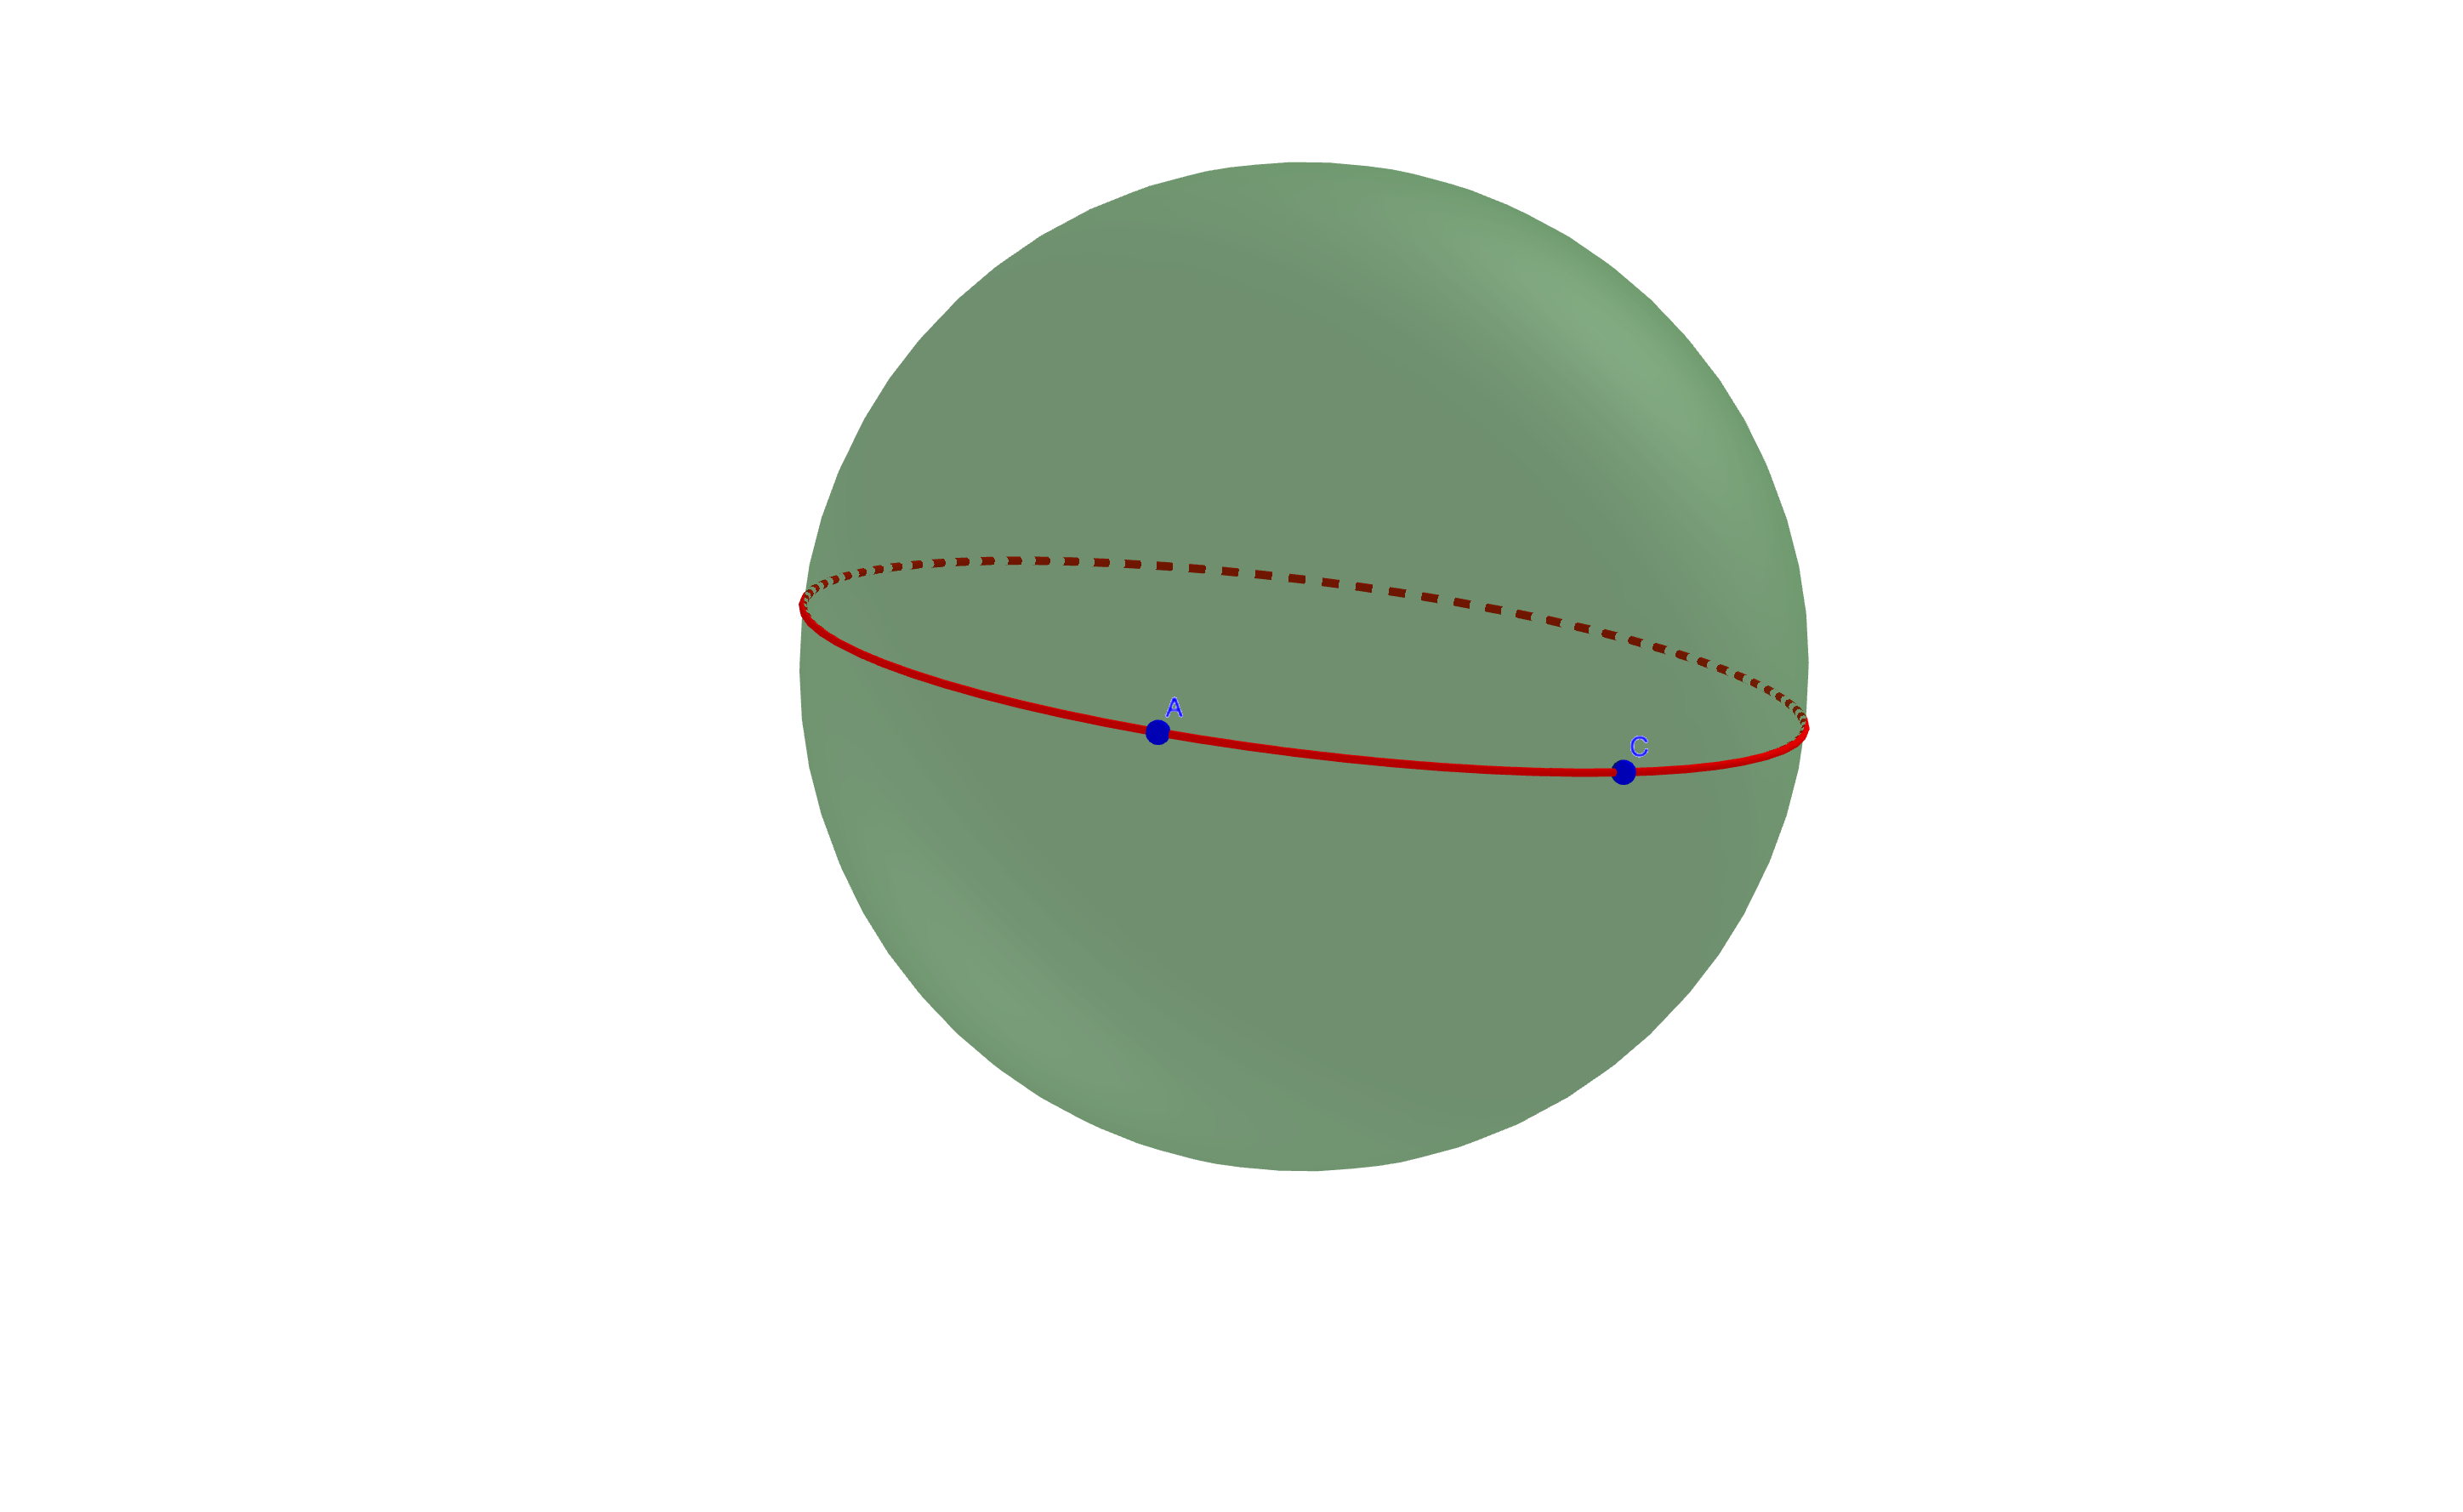
\includegraphics[trim={12cm 12cm 12cm 6cm},clip, width=\textwidth]{oving_1/326.png}
    \end{figure}
  \end{punkt}

  \begin{punkt}
    Dersom $A$ og $C$ er antipodale er $s(A, C)=\pi$ \emph{per definisjon}, ettersom $A$ 
    og $C$ ikke bestemmer en entydig storsirkel. I dette tilfellet er $\overline{AC}$ 
    hele sfæren $S^2$. Hvis vi plukker et tilfeldig punkt $B$ på sfæren, vil $A$, $B$, 
    $C$ alle tre ligge på en felles storsirkel, så det er klart at 
    $s(A,C) = \pi = s(A, B)+s(B, C)$. 
  \end{punkt}
\end{oppgave}


